\chapter{Insertion Sort and Selection Sort}
    \section{Insertion Sort}
    The Insertion Sort algorithm iterates over a list of elements, and at each iteration, it inserts the current element into its correct position in the sorted part of the list (on the left). It works by shifting larger elements one position to the right to make room for the inserted element. The algorithm ensures that the leftmost part of the array, relative to the current index, is always ordered.
    \begin{itemize}
        \item \textbf{Initial array:} A = \{5, 2, 4, 6, 1, 3\}
        \item \textbf{Sorted steps:}
        \begin{itemize}
            \item After first iteration: A = \{2, 5, 4, 6, 1, 3\}
            \item After second iteration: A = \{2, 4, 5, 6, 1, 3\}
            \item After third iteration: A = \{2, 4, 5, 6, 1, 3\}
            \item After fourth iteration: A = \{1, 2, 4, 5, 6, 3\}
            \item After fifth iteration: A = \{1, 2, 3, 4, 5, 6\}
        \end{itemize}
    \end{itemize}
    Note:
    \begin{enumerate}
        \item The leftmost element, with respect to the current index, is always ordered.
        \item When an element is moved from position $j$ to a position $i < j$, the elements from $i$ to $j-1$ must be shifted to make room for it.
        \item If there is only one element the problem is always solved.
    \end{enumerate}
    \subsection{Insertion Sort Pseudo-code}
    The following is the pseudo-code for the Insertion Sort algorithm:
    \begin{verbatim}
    INSERTION-SORT(A)
        for j = 2 to length(A) do
            key = A[j]
            // insert A[j] into the
            // sorted sequence A[1..j-1]
            i = j - 1
            while i > 0 and A[i] > key do
                A[i+1] = A[i]
                i = i - 1
            A[i+1] = key
    \end{verbatim}
    \textbf{Explanation of the steps:}
    \begin{itemize}
        \item We start from the second element in the list and treat the first element as a sorted list.
        \item For each new element, we compare it to the already sorted part and shift larger elements to the right to insert the new element in its correct position.
    \end{itemize}
    
    \subsection{First Iteration Example}
    Consider the array A = \{5, 2, 4, 6, 1, 3\}:
    \begin{itemize}
        \item $j = 2$, $A[2] = 2$, $i = 1$, key = 2
        \item While $i > 0$ and $A[i] = 5 > 2$:
        \begin{itemize}
            \item $A[i+1] = 5 \Rightarrow A = \{5, 5, 4, 6, 1, 3\}$
            \item $i = i-1 = 0$
        \end{itemize}
        \item Exit the loop: $A[i+1] = 2 \Rightarrow A = \{2, 5, 4, 6, 1, 3\}$
    \end{itemize}
    
    \subsection{From Pseudo-code to Python}
    The following is the Python code for Insertion Sort:
    
    \begin{verbatim}
    def insertionSort(A):
        for j in range(1, len(A)):
            key = A[j]
            i = j
            while i >= 0 and A[i-1] > key:
                A[i] = A[i-1]
                i = i - 1
            A[i] = key
    \end{verbatim}
    
    \subsection{Running Time Analysis}
    The running time of an algorithm depends on the size of its input, denoted as $n$. The input size can be defined by the number of items in the input array.
    \begin{figure}[h]
        \centering
        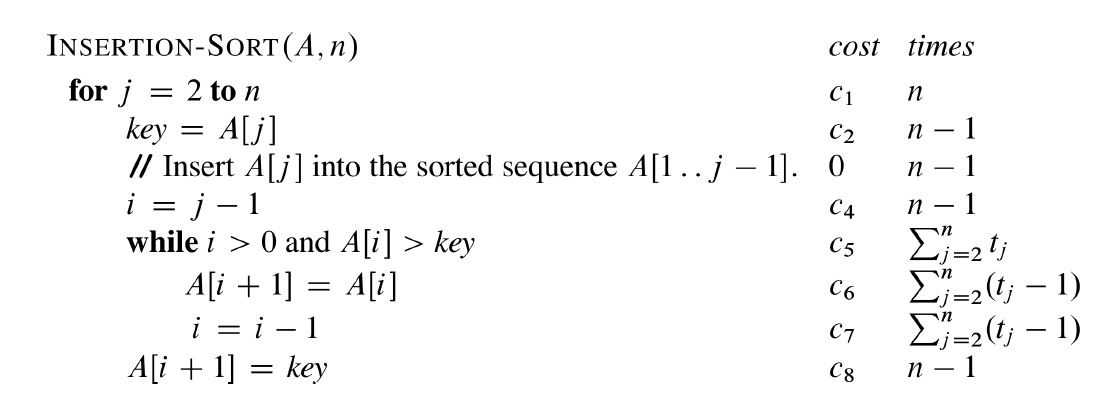
\includegraphics[width=0.9\linewidth]{insertion_sort.png}
    \end{figure}
    
    We are analyzing the time complexity of the \texttt{Insertion-Sort} algorithm. The cost of the algorithm is directly related to the number of times each step is repeated. Let’s go through the steps and calculate their costs.
    
    \subsection{Step-by-Step Cost Analysis}
    
    \begin{itemize}
        \item \textbf{Step 1:} The \texttt{for} loop iterates from $j = 2$ to $n$, so the condition is checked $n$ times, including the final check that fails. Hence, the total cost for this step is $c_1 \cdot n$.
        
        \item \textbf{Step 2:} The body of the \texttt{for} loop is executed $n-1$ times. Thus, this step has a cost of $c_2 \cdot (n-1)$.
        
        \item \textbf{Step 3:} The comment within the code is not executed, so its cost is $0$, even though it is "executed" $n-1$ times. Therefore, $c_3 = 0$.
        
        \item \textbf{Step 4:} The statement $i = j-1$ inside the \texttt{for} loop is executed $n-1$ times, hence the cost is $c_4 \cdot (n-1)$.
        
        \item \textbf{Step 5:} The \texttt{while} loop is nested inside the \texttt{for} loop. The cost depends on how many times the \texttt{while} loop is executed for each $j$, denoted as $t_j$. Therefore, the cost is the sum of $t_j$ from $j=2$ to $n$: 
        \[
        c_5 \cdot \sum_{j=2}^{n} t_j.
        \]
        
        \item \textbf{Steps 6 and 7:} The costs for these steps are also inside the \texttt{while} loop and depend on $t_j-1$, as the condition is not checked after the loop terminates. Hence, the total cost is:
        \[
        c_6 \cdot \sum_{j=2}^{n} (t_j - 1) + c_7 \cdot \sum_{j=2}^{n} (t_j - 1).
        \]
        
        \item \textbf{Step 8:} The assignment $A[i+1] = \texttt{key}$ occurs $n-1$ times, since it's inside the \texttt{for} loop. The total cost for this step is $c_8 \cdot (n-1)$.
    \end{itemize}
    
    \subsection{Overall Time Complexity}
    The total time complexity $T(n)$ of the \texttt{Insertion-Sort} algorithm is the sum of all these contributions:
    \[
    T(n) = c_1 \cdot n + c_2 \cdot (n-1) + 0 + c_4 \cdot (n-1) + c_5 \cdot \sum_{j=2}^{n} t_j + (c_6 + c_7) \cdot \sum_{j=2}^{n} (t_j - 1) + c_8 \cdot (n-1).
    \]
    
    \subsection{Best Case Scenario}
    In the best case, the input sequence is already sorted. This means that for all $j$, $t_j = 1$ (the \texttt{while} loop does not run). The time complexity becomes:
    \[
    T(n) = c_1 \cdot n + c_2 \cdot (n-1) + c_4 \cdot (n-1) + c_8 \cdot (n-1),
    \]
    which simplifies to:
    \[
    T(n) = (c_1 + c_2 + c_4 + c_8) \cdot n - (c_2 + c_4 + c_8).
    \]
    If we denote the constants as $b = c_1 + c_2 + c_4 + c_8$ and $d = -(c_2 + c_4 + c_8)$, the best case complexity is:
    \[
    T(n) = bn + d.
    \]
    In this case, everything inside the \texttt{while} loop is skipped and we assume all the constant equal to 1. Therefore, $T(n) = 5n - 4$.
    
    \subsection{Worst Case Scenario}
    In the worst case, the input sequence is sorted in reverse order. Here, $t_j = j$, which means the \texttt{while} loop executes $j$ times for $j=2,...,n$. The total cost for steps 5, 6, and 7 is:
    \[
    \sum_{j=2}^{n} t_j = \frac{n(n+1)}{2} - 1,
    \]
    and for steps 6 and 7:
    \[
    \sum_{j=2}^{n} (t_j - 1) = \frac{n(n-1)}{2}.
    \]
    Thus, the total time complexity in the worst case becomes:
    \[
    T(n) = c_1 \cdot n + c_2 \cdot (n-1) + c_4 \cdot (n-1) + c_5 \cdot \left(\frac{n(n+1)}{2} - 1\right) + (c_6 + c_7) \cdot \frac{n(n-1)}{2} + c_8 \cdot (n-1).
    \]
    This simplifies to:
    \[
    T(n) = \frac{3}{2}n^2 + \frac{7}{2}n - 4.
    \]
    
    \subsection{General Case}
    In general, the time complexity in the best case is $T(n) = bn + c$, where $b$ and $c$ are real constants, while in the worst case, it is $T(n) = an^2 + bn + c$, where $a$, $b$, and $c$ are real constants.

    \section{Selection Sort}
    Selection Sort is a simple comparison-based sorting algorithm that works by repeatedly selecting the smallest (or largest) element from an unsorted portion of the array and swapping it with the first unsorted element. 
    
    \subsection{Example}
    Consider the array \( A = [2, 5, 6, 4, 1, 3] \). The goal is to sort this array in ascending order using Selection Sort.
    
    \subsection{Steps of the Algorithm}
    \begin{itemize}
        \item Initial Setup: Start with the first element of the array as the current position \( j \) (initially \( j = 1 \)).
        \item Finding the Minimum: Compare the element at smallest with each subsequent element in the array:
        \begin{verbatim}
            For \( i = j + 1 \) to \( n \):
                If \( A[i] < A[smallest] \), update smallest to \( i \).
        \end{verbatim}
        \item Swap: After the inner loop completes, swap the elements at positions \( j \) and smallest.
        \item Repeat: Increment \( j \) and repeat the process until the entire array is sorted.
    \end{itemize}
    
    \subsection{Detailed Example Steps}
    \begin{itemize}
        \item Step 1: \begin{itemize}
            \item \( j = 1 \): \( A = [2, 5, 6, 4, 1, 3] \)
            \item Smallest is initially at index 1 (value 2).
            \item Compare with elements at indices 2 to 6.
            \item Smallest value found at index 5 (value 1).
            \item Swap \( A[1] \) with \( A[5] \):
            \item Result: \( A = [1, 5, 6, 4, 2, 3] \)
        \end{itemize}
        \item Step 2: \begin{itemize}
            \item \( j = 2 \): \( A = [1, 5, 6, 4, 2, 3] \)
            \item Smallest is at index 2 (value 5).
            \item Compare with elements at indices 3 to 6.
            \item Smallest value found at index 5 (value 2).
            \item Swap \( A[2] \) with \( A[5] \):
            \item Result: \( A = [1, 2, 6, 4, 5, 3] \)
        \end{itemize}
        \item Further Steps: Continue this process until \( j = n-1 \).
    \end{itemize}
    
    \subsection{Complexity Analysis}
    Selection Sort has a consistent time complexity of \( O(n^2) \), regardless of the initial order of the elements. This is because the algorithm always examines every element to find the minimum for each position in the array.
    
    There are no best-case or worst-case scenarios that can reduce the complexity since the algorithm must always perform the same number of comparisons.
    
    \subsection{Pseudocode}
    The pseudocode for Selection Sort is as follows:
    
    \begin{verbatim}
    n = length(A)
    for j = 1 to n - 1 do:
        smallest = j
        for i = j + 1 to n do:
            if A[i] < A[smallest] then
                smallest = i
        exchange A[j] with A[smallest]
    \end{verbatim}
    In Python, the exchange can be implemented using a temporary variable:
    \begin{verbatim}
    tmp = A[j]
    A[j] = A[smallest]
    A[smallest] = tmp
    \end{verbatim}
    
    \subsection{Cost Analysis}
    Let's denote the cost of each operation in the pseudocode:
    
    \begin{enumerate}
        \item Step 1 is executed once: \( 1 \)
        \item Step 2 is executed \( n \) times: \( n \)
        \item Step 3 is executed \( n-1 \) times: \( n - 1 \)
        \item Steps 4 and 5 are the sum of \( j \) from \( 1 \) to \( n-1 \): \( \sum_{j=1}^{n-1} t_j \)
        \item Steps 6 is the sum of \( j \) from \( 1 \) to \( n-1 \): \( 2 \sum_{j=1}^{n-1} (t_j - 1) \)
        \item Step 7 is executed \( n - 1 \) times: \( n - 1 \)
    \end{enumerate}
    The total cost \( T(n) \) in operations is given by:
    \[
    T(n) = 1 + n + (n - 1) + \sum_{j=1}^{n-1} t_j + 2 \sum_{j=1}^{n-1} (t_j - 1) + (n - 1)
    \]
    Using the steps for Insertion Sort, we can derive that:
    \[
    T(n) = 3n - 1 + \frac{n(n-1)}{2} + n(n-1) - 1
    \]
    Thus, the complexity of Selection Sort is in the order of \( O(n^2) \), it's remains the same for the best and worst case since we have to do the two for loops.
    
    \section{When to Use Selection Sort vs Insertion Sort}
    Selection Sort is generally not stable and does not perform well on large datasets due to its \( O(n^2) \) complexity. However, it has the advantage of performing a constant number of swaps, making it useful when memory writes are costly. \newline
    Insertion Sort, on the other hand, is more efficient for smaller datasets or partially sorted arrays, as it has a best-case time complexity of \( O(n) \) when the array is already sorted. Thus, Insertion Sort is preferable when dealing with nearly sorted data or small lists. In the best case Insertion sort is only $\Theta(n)$ since it doesn't enter the while loop.
